\documentclass[fleqn]{VUMIFPSkursinis}
\usepackage{algorithmicx}
\usepackage{algorithm}
\usepackage{algpseudocode}
\usepackage{amsfonts}
\usepackage{amsmath}
\usepackage{bm}
\usepackage{caption}
\usepackage{color}
\usepackage{float}
\usepackage{graphicx}
\usepackage{listings}
\usepackage{subfig}
\usepackage{wrapfig}

% Titulinio aprašas (nereikalingus elementus užkomentuoti)
\university{Vilniaus universitetas}
\faculty{Matematikos ir informatikos fakultetas}
% \institute{Informatikos institutas}  % Užkomentavus šią eilutę - institutas neįtraukiamas į titulinį
\department{Programų sistemų bakalauro studijų programa}
\papertype{Kursinis darbas}
\title{Migracijos strategijos migruojant iš monolitinės į mikroservisų architektūrą}
\titleineng{Strategies for migrating from monolith to microservices architecture}
\author{Audrius Kumpis}
\status{4 kurso, 2 grupės studentas}
\supervisor{lekt. Vasilij Savin}
\date{Vilnius \\ \the\year}

% Nustatymai
\captionsetup{justification=centering}
% \setmainfont{Palemonas}  % Pakeisti teksto šriftą į Palemonas (turi būti įdiegtas sistemoje)
\bibliography{bibliografija}  % Literatūros šaltinių aprašų failas bus bibliografija.bib

\begin{document}
\maketitle

\tableofcontents

\sectionnonum{Santrauka}
Monolitinės aplikacijos migravimas į mikroservisų architektūrą gali būti itin sudėtingas ir daug planavimo reikalaujantis uždavinys \cite{FBZ+19}. Privaloma atlikti nuoseklų darbų bei būsimo dizaino planavimą, kad migravimas būtų atliktas sėkmingai. Šiame darbe yra palyginti trys metodai, kurių pagalba yra galima atlikti pertvarkymo darbus: dekomponavimas skaidant domenus, visiškas sistemos perdarymas ir dirbtiniu intelektu paremtas įrankis „Mono2Micro“. Taip pat yra aptarta monolitinės duomenų bazės skaidymo problema. Metodų lyginimas yra fokusuotas į įvairias metrikas, kaip programinio kodo dydis ar priklausomybė nuo padengiamumo funkciniais testais. Darbe yra parodyta, jog kiekvienas metodas turi savo pranašumų ir trūkumų, ir kad pats efektyviausias metodas yra priklausomas nuo sistemos specifinių charakteristikų ir reikalavimų, bei nuo trokštamos mikroservisų architektūros dizaino. Darbo metu parodyta, jog dekomponavimo pagal domenus ir „Mono2Micro“ metodų kombinacija yra tinkamiausias būdas pertvarkyti monolitinę sistemą. Darbo rezultatas – empiriniu būdu  palyginti metodai ir tinkamiausio metodo parinkimas praktiniam realizavimui bakalauro baigiamajame darbe.

\sectionnonum{Summary}
The process of refactoring a monolithic application to a microservices architecture can be complex and requires careful planning and design to ensure the success of the migration \cite{FBZ+19}. This study compares three approaches for refactoring a monolithic application to a microservices architecture: domain-driven design, re-architecture, and the AI tool Mono2Micro. Monolithic database refactoring is also covered in this study. Evaluation focuses on a variety of metrics, including codebase size or dependency on code coverage. It is found that each approach has its own strengths and limitations, and that the most effective approach may depend on the specific characteristics and requirements of the monolithic application and the desired microservices architecture. The results suggest that a combination of domain-driven design and AI-assisted refactoring can be a powerful tool for migrating monolithic applications to microservices, and can help organizations achieve the benefits of a microservices architecture while minimizing the risks and challenges of the refactoring process. Overall result of the article – an empirical evaluation of different approaches and a prepared data for realisation in the Bachelor‘s Thesis.
% \keywords{keyword 1, keyword 2, keyword 3, keyword 4, keyword 5}


\sectionnonum{Įvadas}
Kai komanda pradeda kurti programą, monolitas įprastai yra numatytas pasirinkimas. Tai yra viena pagrindinių priežasčių, kodėl egzistuoja itin daug monolitinių sistemų. Monolitas turi savo duomenų bazę, savo funkcionalumo įgyvendinimą ir tai yra vientisa programa. Jis yra lengvai suprogramuojamas ir su palyginamai nedideliu darbo indėliu, galima greitai sukurti bei diegti veikiančią sistemą. Tačiau tokią architektūrą yra labai sunku plėtoti bei palaikyti. Kuo daugiau  tokia sistema yra plėtojama, tuo daugiau ji didėja, daugėja kodo bei priklausomybių nuo kitų sistemų. Diegimai tampa ilgi ir itin reti. Testavimas būna sudėtingas, nes negalima atlikti izoliuoto atskirų sistemos modulių testavimo. Kad ši problema būtų išspręsta, paprastai monolitinės sistemos yra skaidomos į mikroservisus.

Mikroservisai – tai atskiri, nedideli servisai, kurie atsakingi už tam tikras specifines užduotis. Jie yra implementuoti kaip atskiros programos, o komunikacija tarp jų įprastai yra vykdoma per pranešimų siuntimo (angl. messaging) technologijas arba per REST API. Kiekvienas mikroservisas turi savo duomenų bazę, savo diegimo strategijas bei testavimo aplinką. Mikroservisų architektūra suteikia daug privalumų, pavyzdžiui:
\begin{itemize}
    \item Pagreitinami sistemos diegimai.
    \item Pagerinamas sistemos plečiamumas.
    \item Nėra priklausomybės nuo pasirinktų technologijų.
    \item Prie sistemos implementacijos gali dirbti didesnis komandų skaičius.
\end{itemize}

Nors mikroservisai išsprendžia daug problemų, tai nėra paprastas sprendimas. Kadangi migravimas į mikroservisų architektūrą yra pilnai techninė užduotis, privaloma gauti projekto vadovo ir/ar projekto savininko sutikimą, kad migracijai būtų skiriami resursai bei lėšos. Viena iš sunkesnių migracijos dalių yra mikroservisų projektavimas. Yra daugybė būdų, kaip galima išskaidyti monolitinę sistemą į mažesnius servisus \cite{FBZ+19}, taigi iš anksto apgalvoti, kokia strategija bus taikoma yra svarbu ir laiko, ir resursų atžvilgiu. Kad migracija iš monolitinės architektūros į mikroservisų būtų sklandi, reikia gerai žinoti, kokius darbus ir kokia tvarka būtina atlikti. Jau egzistuoja keletas migravimo atlikimo strategijų \cite{Wal22,MQO18,KXL+20}, su kuriomis susipažinus yra lengviau suplanuoti reikiamus darbus. Šiame darbe bus aptartos šios strategijos:
\begin{itemize}
    \item Dekomponavimas skaidant domenus.
    \item Visiškas sistemos perdarymas.
    \item Dekomponavimas naudojant dirbtiniu intelektu paremtą įrankį „Mono2Micro“.
\end{itemize}

\sectionnonum{Darbo tikslas ir uždaviniai}
Darbo tikslas: įvertinti šias tris monolitinės sistemos skaidymo į mikroservisų architektūrą strategijas, siekiant surasti optimaliausią variantą, kuris būtų lengviausiai pritaikomas ir neatnešantis didelių nuostolių laiko ir naudojamų resursų atžvilgiu. Kad šis tikslas būtų pasiektas, kiekviena strategija bus aprašyta ir bus įvertinamas jų teorinis pritaikymas. Kiekvienas skyrius bus baigiamas pastebėjimais ir rekomendacijomis aptariamai strategijai. Po rezultatų analizės bus parodyta, kokia strategija, ar strategijų kombinacija, yra veiksmingiausia monolito migravimo į mikroservisų architektūrą užduočiai.

\section{Dekomponavimas skaidant domenus}
Pirmiausia aptarsime vieną iš populiariausių migravimo strategijų – skaidymas pagal domenus \cite{Wal22}. Šią strategiją verta naudoti tuomet, kai verslo panaudos sritys yra aiškiai išskirtos. Dažnai  ši sąlyga būna neįgyvendinta, todėl yra itin svarbu į monolito pertvarkymo procesą įtraukti verslo atstovus, analitikus bei kitus techninius sistemos atstovus, kurie gerai supranta perdaromos sistemos funkcionalumą esančiame įgyvendinime.

\subsection{Strategijos aprašymas}
Dekomponavimas skaidant domenus (angl. domain-driven refactoring) yra viena iš populiariausių migravimo strategijų. Ją geriausia naudoti tuomet, kai monolitas buvo kurtas laikantis domenais paremtu kūrimu (angl. domain-driven development). Tačiau ne visada būna taip, jog monolitas yra jau iš karto paruoštas migravimui. Pirmas ir svarbiausias žingsnis yra esminių domenų identifikavimas \cite{LZ22}. Kad esminių domenų identifikavimas būtų atliktas sėkmingai, privaloma įtraukti visus suinteresuotuosius asmenis minėtus anksčiau. Kad nauja architektūra tinkamai atliktų užduotis, privaloma investuoti laiko į monolito servisų sėkmingą migravimą į atskirus servisus. 

Šios problemos sprendimas buvo pristatytas 2011 metais, o mikroservisų idėja buvo pristatyta 2005 metais. Sprendimo idėja yra paprasta: kai naujo domeno funkcionalumas yra įgyvendintas mikroservise ir jau yra paruoštas naudojimui, sistema perima naujojo mikroserviso funkcionalumą ir nebenaudoja jo iš senosios sistemos. Tai yra daroma su kiekvienu esminiu, atrinktu domenu. Tokiu būdu, monolitas yra „smaugiamas“ tol, kol jame nebebus nei vieno naudojamo domeno. Iš to ir seka šios taktikos pavadinimas – „Smaugiko šablonas“ \cite{Beh18}. Šis šablonas yra taikomas beveik visuomet, kai yra naudojamas dekomponavimo pagal domenus strategija.

\subsection{Strategijos pritaikymas}
Šiame pavyzdyje naudojama fiktyvi paskolų išdavimo sistema. Šioje sistemoje yra naudojami 5 esminiai domenai: autentikacijos, paskolos dydžio skaičiuoklė, išmokėjimo mechanizmas, kreditingumo skaičiuoklė, transakcijų gavimo mechanizmas. Visi šie domenai veikia darnoje ir yra priklausomi vienas nuo kito. Jų veikimas pavaizduotas šioje diagramoje:
\begin{figure}[H]
    \centering
    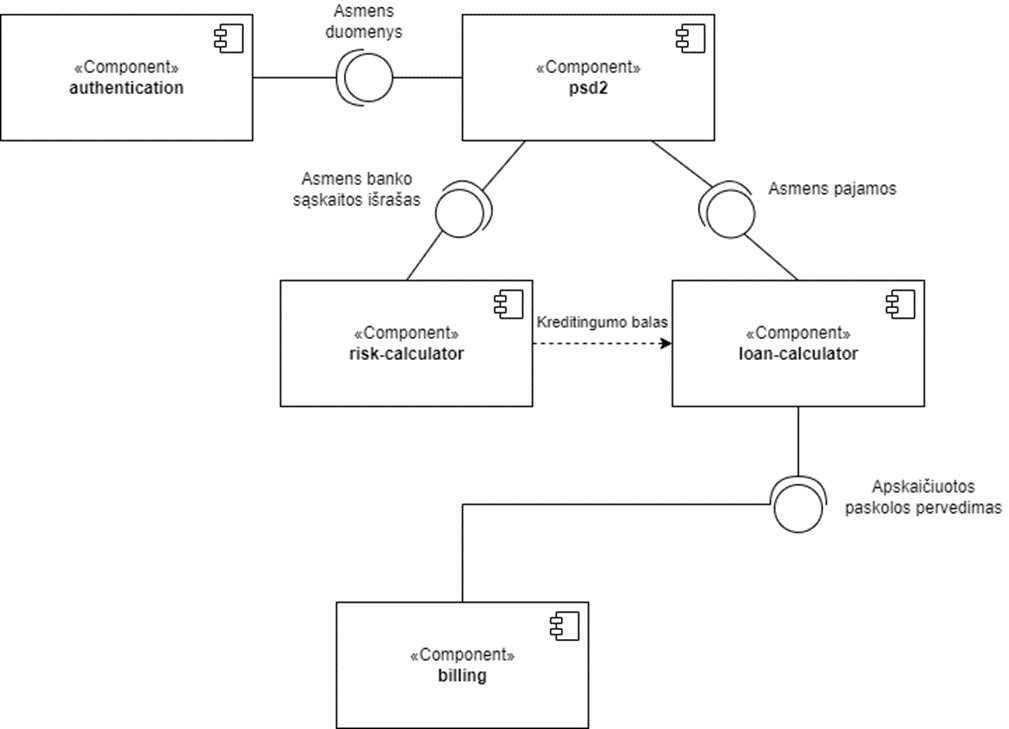
\includegraphics[scale=0.9]{img/komponentu-diagrama.png}
    \caption{Dabartinio monolito komponentų diagrama}
    \label{img:komponentu-diagrama}
\end{figure}

Visi šie domenai – komponentai – priklauso vienas nuo kito. Jei bent vienas neveikia, arba veiks klaidingai, tai atneš nenumatytų nuostolių verslui. Pasinaudojant „smaugiko“ šablonu, iteratyviai kiekvienam išskirtam domenui, yra sukuriamas mikroservisas. Kūrimo metu yra privaloma užtikrinti, jog bendras sistemos veikimas nėra sugadinamas, jog sistema vis dar veikia korektiškai. Kad tai būtų užtikrinta, privaloma kuo anksčiau sukonfigūruoti pastovaus diegimo/pastovaus testavimo liniją. (angl. CI/CD pipeline)  Supaprastintą šablono panaudojimą galima pamatyti \ref{img:smaugiko-sablonas} pav.

\begin{figure}[H]
    \centering
    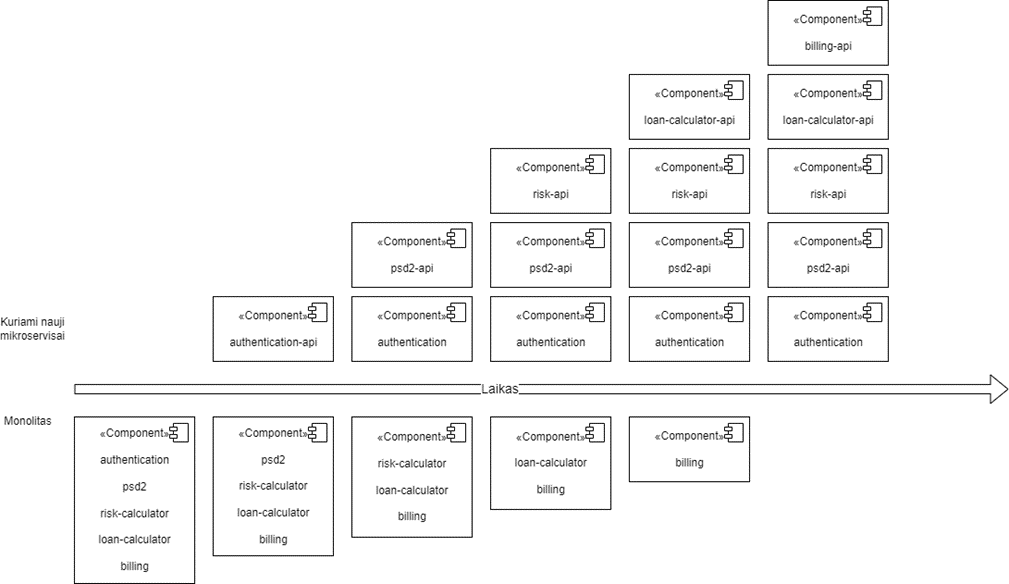
\includegraphics{img/smaugiko-sablonas.png}
    \caption{„Smaugiko“ šablono įgyvendinimas}
    \label{img:smaugiko-sablonas}
\end{figure}

Naujai sukurtiems mikroservisams yra būtina kuo anksčiau priskirti atsakingas komandas. Šios komandos bus atsakingos už tolimesnius mikroservisų darbus, priežiūrą, keitimus, bei teisingos integracijos su dar laikinai naudojamu monolitu užtikrinimą. Taigi prieš visą migraciją privaloma įsivertinti, ar programavimo komandoje pakanka resursų priskirti žmones specifiniams mikroservisams.

Iš karto gali kilti klausimas: kaip atsirinkti, ką pirmiausia reikia iškelti į naują mikroservisą? Jei šis šablonas yra taikomas pirmą kartą programavimo komandoje, saugiausias variantas būtų pradėti nuo mažiausiai reikšmingo ir/ar mažiausio pagal dydį komponento. Tokiu būdu, komanda įgautų daugiau patirties darbui labiau svarbiems komponentams. Be šito, kiti galimi kandidatai yra \cite{Beh18}:
\begin{itemize}
    \item Komponentai, kurie yra labiausiai užbaigti. Jie turi didžiausią padengimo testais procentą, mažiausiai neužbaigtų techninių darbų. Programavimo komanda tuomet jaustųsi saugiausiai migruodama šį komponentą.
    
    \item Komponentai, kurie tikėtina, jog plėsis labiausiai. Iškėlus juos į mikroservisus pirmiausia, tikėtina, jog reikės perkelti mažiau kodo, nei tą darbą atliekant vėliau.
    
    \item Komponentai, kurie dažniausiai kinta dėl besikeičiančių verslo reikalavimų. Tai užtikrintų, jog atliekant verslo reikalaujamus pakeitimus, nereiktų diegti viso monolito, užtektų diegti tik naują mikroservisą.\\
\end{itemize}

\subsection{Įvertinimas}
Taigi, šią migravimo strategiją rekomenduojama naudoti tuomet, kai yra aiškiai apibrėžti domenai, arba jei yra galimybė įtraukti verslo atstovus aiškių esminių domenų identifikavimui. Tačiau ši strategija nėra tinkama visiems atvejams. Jos nerekomenduojama naudoti tuomet, kai monolitas yra dar itin mažos apimties ir neturi aiškiai apibrėžtų esminių domenų. Priešingu atveju, gali būti brangu sumodeliuoti, kurti bei prižiūrėti naujai sukurtus mikroservisus. Naudojantis šia strategija, atliekamo pertvarkymo darbo laikas tiesiogiai priklauso nuo esamo monolito dydžio. Kuo didesnis monolitas, tuo ilgiau truks jį išskaidyti. Sunkiausia dalis visgi lieka esminių domenų identifikavimas. Taip pat, jei esamame monolite yra didelis kodo padengimas funkciniais testais, tai gali padėti užtikrinti, jog migravimas bus sėkmingas ir reikės atlikti mažiau pilno testavimo rankiniu būdu.

\section{Pilnas sistemos perdarymas}
Nors tai dažnai yra laikoma kraštutine strategija, ją taip pat yra būtina paminėti. Kai esama sistema neatlieka savo verslo funkcijų tinkamai, kai sistemą yra sunku naudoti arba kai sistema yra sukurta naudojant pasenusiomis technologijomis, tada šį monolito migravimo būdą verta apmąstyti \cite{MQO18}.

\subsection{Strategijos aprašymas}
Priežasčių pilnam sistemos perdarymui gali būti daug, pavyzdžiui:
\begin{itemize}
    \item Aukšti esamos sistemos palaikymo kaštai \cite{Gli21}. Senoms sistemoms reikia daugiau jas gebančių palaikyti specialistų. Jei monolitas buvo sukurtas su jau pasenusiomis technologijomis, tokių specialistų atrasti gali būti sunku. Jei ir randami šie specialistai, jie bus priskirti prie projekto palaikymo komandos ir tik prižiūrės esamą sistemą, kuri gali veikti klaidingai, arba visai neveikti.
    
    \item Nepritaikymas esamiems įstatymams. Jei yra išleidžiami nauji įstatymai, kurie apriboja buvusius sistemos panaudos atvejus, esamą monolitinę sistemą pritaikyti pagal tuos įstatymus gali būti labai sudėtinga. Potencialiai, jie gali pakeisti visą verslo logiką, duomenų struktūrą.
    
    \item Pasenusios technologijos \cite{MQO18}. Surasti specialistus, kurie sugeba palaikyti sistemą, kuri buvo sukurta su senomis technologijomis, gali būti labai sudėtinga. Tokiu atveju sėkmingas verslo užduočių veikimas  yra itin priklausomas nuo specialistų, kurie dirba įmonėje. Idealiu atveju, verslo veiksmingumas neturėtų priklausyti nuo tokių faktorių. Taip pat, senos technologijos reiškia pasenusius saugumo standartus. Sistema tampa mažiau saugi naudoti ir, natūraliai, mažiau patraukli būsimiems ir esamiems vartotojams.\\
\end{itemize}

Įvertinus esamą sistemą, galima apgalvoti apie sprendimą ją perdaryti ir tuo pačiu pereiti prie mikroservisų architektūros. Bendru atveju, sistemos perdarymas yra vienodai sudėtingas darbas, lyginant su naujos sistemos sukūrimu, taigi yra būtina gauti visos komandos, produkto savininko, projekto vadovo ir kitų suinteresuotųjų asmenų pritarimą sistemos perdarymui. Po įvykdomumo analizės bei reikalavimų surinkimo, belieka įvykdyti sistemos perdarymą. Vykdymas gali būti daromas daugeliu būdų, tačiau čia yra aprašyti du populiariausi metodai: „didžiojo sprogimo“ \cite{Ngu11} metodas ir patobulintas perdarymo mechanizmas \cite{MQO18} (angl. enhanced re-engineering mechanism).

\subsection{Strategijos pritaikymas}
„Didžiojo sprogimo“ metodo idėja yra paprasta. Pagrindinis tikslas yra perdaryti visą sistemą vienu metu. Šis metodas įprastai yra pasirenkamas, kai projekto problemą reikia išspręsti kuo greičiau, pvz., pakeisti sistemos architektūrą \cite{Ngu11}. Šis metodas yra itin lankstus, galima atsisakyti nereikalingų sąsajų, galima iš karto prisitaikyti prie naujos diegimo aplinkos. Tačiau šio metodo pritaikymas labai priklauso nuo konkretaus projekto. Metodas netinka labai didelėms sistemoms, nes sunaudojama labai daug resursų. Naudojant šį metodą rizika, jog projektas–perdarymas nepasiseks yra didelė, nes visas procesas trunka panašiai tiek pat ilgai, kaip kuriant visiškai naują sistemą.
\begin{figure}[H]
    \centering
    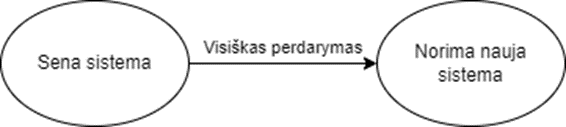
\includegraphics{img/didziojo-sprogimo-metodas.png}
    \caption{„Didžiojo sprogimo“ metodas}
    \label{img:didziojo-sprogimo-metodas}
\end{figure}

Patobulintas perdarymo mechanizmas yra labiau struktūrizuotas procesas, savo žingsniais primenantis klasikinį programų kūrimo procesą. Pirma, yra atliekama įvykdomumo analizė, o tada surenkami reikalavimai naujai sistemai. Turint naujus reikalavimus, pereinama prie programavimo fazės. Atlikus programavimą, atliekamas testavimas, naujų algoritmų palyginimas su sena sistema, naujų technologijų siūlymai ir pakartotinis testavimas. Procesas tęsiasi tol, kol bus pasiektas norimas atnaujinimo lygis. Šis metodas sumažina sistemos perdarymo kompleksiškumą, pagerina naujai perdarytą sistemą ir užtikrina, jog visi reikiami komponentai bus sėkmingai suintegruoti.

\begin{figure}[H]
    \centering
    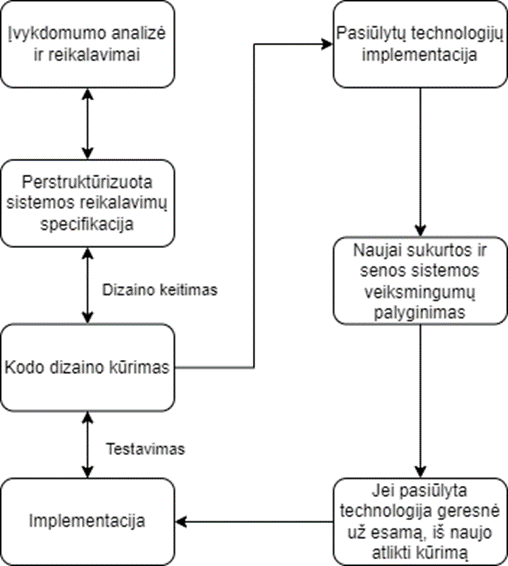
\includegraphics{img/patobulintas-perdarymas.png}
    \caption{Patobulintas perdarymo mechanizmas \cite{MQO18}}
    \label{img:patobulintas-perdarymas}
\end{figure}

\subsection{Įvertinimas}
Visiškas sistemos perdarymas dažnu atveju yra kraštutinė monolito migravimo priemonė, tačiau tinkamomis sąlygomis šis metodas atneša daugiau naudos nei tradicinės monolito migravimo strategijos. Pastebėjus didelį kiekį problemų su esama sistema, galima apmąstyti ne tik apie esamo monolito modernizavimą, bet ir migravimą į mikroservisų architektūrą. Tačiau nedidelis kiekis įmonių yra linkusių pasinaudoti šiuo migravimo metodu, nes jis yra itin ilgai trunkantis ir kainuoja daug resursų \cite{MQO18}. Pastebėta, jog yra modernizavimui skirtų įrankių trūkumas. Jei trūkumo nebūtų, tai galėtų paskatinti esamų senų sistemų modernizavimą ir pertvarkymą į mikroservisų architektūrą.

\section{Dekomponavimas naudojant „Mono2Micro”}
Per pastaruosius metus šis metodas pritraukė daug dėmesio. Jo pagalba galima palengvintu būdu atskirti esminius domenus bei juos iškelti į naujus mikroservisus. Naudojantis šiuo įrankiu klaidų tikimybė yra tikėtinai mažesnė, monolito migravimas tampa greitesnis už tradicinius metodus bei turi galimybę paruošti naujus mikroservisus būti naudojamiems debesijoje (angl. cloud computing). Šio darbo rašymo metu, įrankis sėkmingai atlieka migravimo užduotis tik su Java kalba parašytoms programoms, tačiau ateityje yra numatoma apjungti ir kito tipo programas \cite{KXL+20}.

\subsection{Strategijos aprašymas}
„Mono2Micro“ (toliau įrankis) yra dirbtinio intelekto pagalba sukurtas įrankių rinkinys, kuris padeda pertvarkyti esamą seną sistemą į mikroservisų architektūrą. Įrankis leidžia vartotojui pasirinkti norimus panaudos atvejus ir veikimo metu juos priskirti esančioms klasėms, servisams. Įrankis taip pat atlieka statinę programos analizę ir surenka programos struktūrinę informaciją bei priklausomybes. Šią informaciją tuomet analizuoja dirbtinio intelekto variklis ir sukuria programos padalinius (angl. partitions) pagal verslo panaudos atvejų ir priklausomybių panašumą bei panaudojimą. Sugeneruoti padaliniai yra potencialūs kandidatai naujam mikroservisui. Vartotojas gali peržiūrėti šiuos padalinius, juos redaguoti ar kitaip grupuoti, kad būtų gautas kuo tikslesnis norimas mikroservisas \cite{KXK+21}. Taip pat, kartu su verslo panaudos atvejais, įrankis sugeneruoja natūraliai panašius padalinius. Jie skiriasi tuo, jog nėra analizuojama duomenų priklausomybė. Taip galima supaprastinti duomenų priklausomybes tarp sugeneruotų padalinių.

\begin{figure}[H]
    \centering
    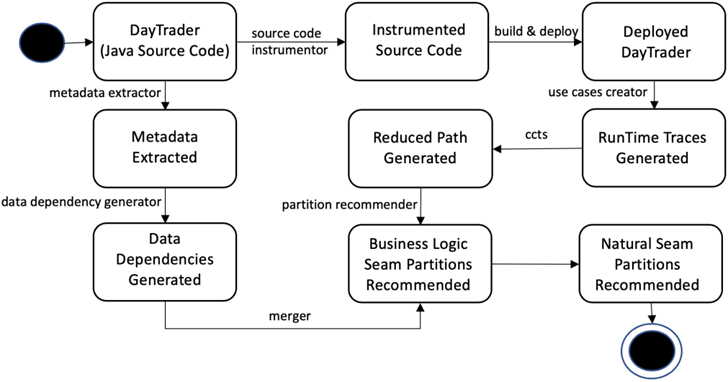
\includegraphics{img/mono-2-micro-veikimas.png}
    \caption{Verslo panaudos atvejų ir natūraliai panašių padalinių generavimas naudojantis „Mono2Micro“ įrankiu \cite{KXL+20}.}
    \label{img:mono-2-micro}
\end{figure}

Kad įrankis sugeneruotų tikslius panaudos atvejus, programa kurią norima pertvarkyti yra paleidžiama. Kai ji pradeda veikti, per vartotojo sąsają būtina atlikti visus panaudos atvejus. Jei kuris nors atvejis bus praleistas, įrankis ieškos daugiau panaudos atvejų funkciniuose testuose. Visa ši informacija yra surenkama į orientuotą grafą $(V, E)$. kur $V$ yra klasės, $E$ yra veikimo metu nustatyti metodų kvietimo sąryšiai tarp klasių \cite{KXL+20}. Sugeneruoto grafo pavyzdys parodomas \ref{img:mono-micro-grafas} pav.

\begin{figure}[H]
    \centering
    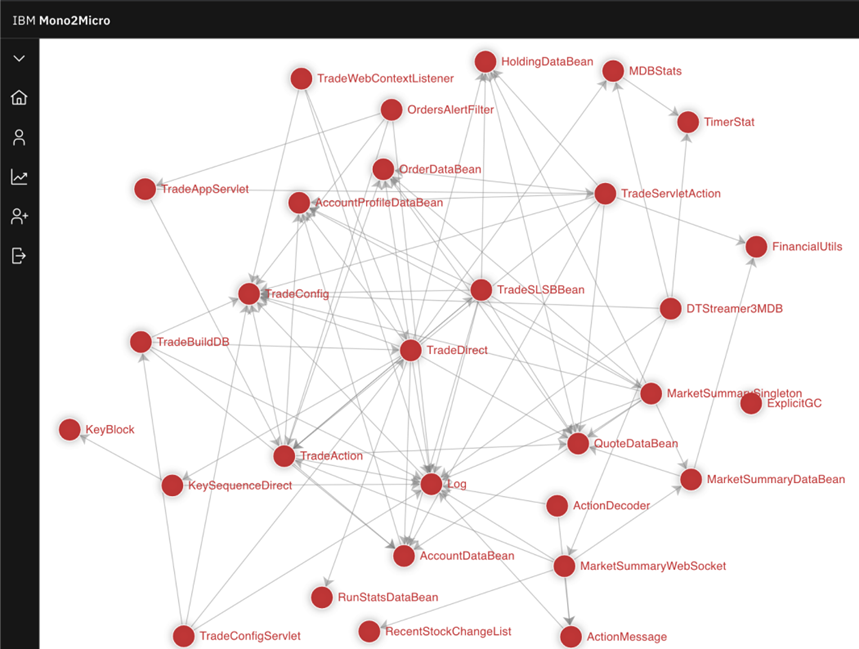
\includegraphics{img/mono-micro-grafas.png}
    \caption{Veikimo metu sugeneruotas orientuotas grafas $(V, E)$, parodantis dinaminius sąryšius tarp klasių \cite{KXL+20}.}
    \label{img:mono-micro-grafas}
\end{figure}

Surinkus visą reikiamą informaciją apie klases ir jų ryšius, įrankis gali pasinaudoti šiais duomenimis bei sugeneruotu kvietimo konteksto medžiu (angl. calling-context tree), kad sukurtų padalinių rekomendacijas. Turint norimą padalinių skaičių $k$ ir klasių aibę $C = {c_{1}, c_{2}, ..., c_{n}}$ galima sugrupuoti klases pasinaudojant šia panašumo formule \cite{KXL+20}.

\begin{equation}\label{eq:panasumo-formule}
    Sim_{i,j} = \frac{\sum_{m=o}^{n_{i}}\sum_{n=0}^{n_{j}}S(c_{im},C_{jn})}{\left| C_{i} \right|\left| C_{j} \right|}
\end{equation}

Panašumo dydis yra apskaičiuojamas remiantis tiesioginiais ir netiesioginiais kvietimų ryšiais tarp klasių $c_{i}$ ir $c_{j}$. Tiesioginio kvietimo ryšys egzistuoja tik tuomet, kai ryšys tarp klasių $c_{i}$ ir $c_{j}$ kvietimo konteksto medyje egzistuoja briauna $(c_{i}, c_{j})$. Netiesioginio kvietimo ryšys tarp klasių $c_{i}$ ir $c_{j}$ egzistuoja tik tuomet, jei konteksto kvietimo medyje egzistuoja kelias $(c_{i}, c_{2}, ..., c_{p}, c_{j}), p > 1$.

Kai yra sugeneruojami padaliniai pagal panaudos atvejų panašumą, įrankis juos sujungia pagal natūralų panašumą. Jei klasės $c_{i}$ ir $c_{j}$ turi ryšių, jos yra priskiriamos vienam padaliniui. Tokiu būdu pereinama per visas visų padalinių klases ir gaunamas optimalus natūraliai panašių padalinių skaičius.

\subsection{Strategijos pritaikymas}
Šiai strategijai išbandyti naudojama populiari „IBM“ sukurta etaloninė programa „DayTrader“ \cite{IBM15}. Tai yra elektroninė akcijų pirkimo ir pardavimo programa. Ji leidžia vartotojui prisijungti, peržiūrėti savo profilį, peržiūrėti esamas akcijas, jų kainas bei kainų istoriją, pirkti bei parduoti akcijas. Joje yra 112 klasių ir 964 metodų. Kodo padengimas funkciniais testais: padengta  66 \% klasių, 44 \% metodų. Pasinaudojus įrankiu ir nurodžius padalinių skaičių $k = 7$ gauname rekomenduojamus 3 padalinius $p_{1}, p_{2}, p_{3}$.

\begin{figure}[H]
    \centering
    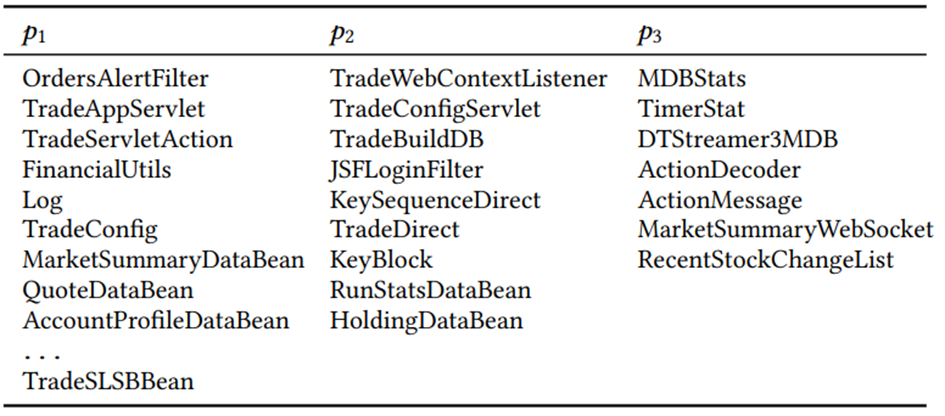
\includegraphics{img/mono-micro-padaliniai.png}
    \caption{Sugeneruoti padaliniai „DayTrader“ programai, kai $k = 7$, \cite{KXK+21}}
    \label{img:mono-micro-padaliniai}
\end{figure}

Padalinyje $p_{1}$ yra priskiriamos klasės, susijusios su akcijų pirkimo ir pardavimo funkcionalumu, $p_{2}$ yra priskiriamos klasės, susijusios su duomenų bazės operacijomis, o $p_{3}$ yra priskiriamos klasės susijusios su įvairių pranešimų siuntimu. Šie padaliniai buvo suskirstyti pagal atliekamas programines funkcijas ir jie nėra glaudžiai susiję su verslo moduliais pasinaudojant įrankio padalinių sujungėju. Parodžius šiuos rezultatus programinės įrangos architektams, kurie yra susipažinę su šia programa, jie patvirtino, jog šie „Mono2Micro“ sugeneruoti mikroservisų patarimai yra logiški ir prasmingi \cite{KXL+20}.\\

\subsection{Įvertinimas}
„Mono2Micro“ tinka sugeneruoti esamo Java EE monolito pertvarkymo rekomendacijoms. Šis įrankis yra lankstus, suteikiantis daug patarimų ir rekomendacijų, ir parodė, jog veikia gerai su vidutinio dydžio Java Spring programomis \cite{San21}. Tačiau įrankis daugiau dėmesio skiria sugrupuoti esamas klases pagal jų techninį funkcionalumą, o ne pagal verslo panaudos atvejus, kas yra įprastas mikroservisų tikslas. Taip pat pastebėtina, jog šis įrankis gali būti naudojamas ne tik monolito paruošimui mikroservisų architektūrai, bet ir patikrinimui, ar monolitą tikrai verta skaldyti į atskirus mikroservisus. Jei gaunamas rekomenduotinų padalinių skaičius yra nedidelis (pvz., 2), tai verta pamąstyti, ar apsimoka skirti laiko ir resursų šiam sudėtingam darbui. Nors šis įrankis šiuo metu veikia tik su Java programomis, tikėtina, jog jis ateityje palengvins ir kitokio tipo programų pertvarkymą.

\section{Monolitinės duomenų bazės skaidymas}
Aprašytos strategijos labiau koncentravosi į pačios monolitinės sistemos dekomponavimą, tačiau nebuvo paminėta, kaip pertvarkyti monolitinę duomenų bazę. Monolitinėje sistemoje, kaip ir bet kurioje kitoje, duomenys yra itin svarbi dalis, tad jų tvarkymas bei duomenų vientisumo užtikrinimas yra kritinė monolito migravimo į mikroservisų architektūrą dalis.

\subsection{Duomenų bazių skaidymo problema}
Praėjusiuose skyriuose buvo aptartas domenais remtas sistemų kūrimas. Jis taip pat gali būti taikomas ir duomenų bazių projektavimui. Anot H. Chawla et al., kiekvienas mikroservisas turėtų turėti atskirą privačią duomenų bazę, nes duomenų prieigos atskyrimas geriausiai leidžia atskiroms technologijoms vykdyti verslo užduotis \cite{CK19}. Jei yra laikoma, jog kiekvienas mikroservisas yra atskiras esminis domenas, tai kiekvienam esminiam domenui turi būti atskirta duomenų bazė.

Monolitinėje sistemoje duomenys yra itin priklausomi vieni nuo kitų, taigi migruojant duomenis į atskiras duomenų bazes, tarp kurių komunikacija nebebus tokia laisva, privaloma užtikrinti, kad duomenys yra korektiškai migruojami į atskiras duomenų bazes ir lenteles. Tai yra itin sudėtingas uždavinys, reikalaujantis didelio atidumo bei nagrinėjamos sistemos išmanymo. Šios problemos vienas populiariausių sprendimo būdų yra duomenų bazės skaidymas identifikavus ribotus kontekstus (angl. bounded contexts) \cite{New19}.

\subsection{Migravimas pagal ribotus kontekstus}
Ribotieji kontekstai yra naudojami, kai norima identifikuoti tokias sistemos dalis, kurios turi unikalius ir nepriklausomus verslo panaudos atvejus \cite{New19}. Kad riboti kontekstai būtų nustatyti, galima analizuoti sistemos verslo reikalavimus, panaudos atvejus, ar panaudos atvejų istorijas. Turint šiuos kontekstus, galima suprasti, kokie duomenys priklauso kokiam mikroservisui. Nustačius ribotus kontekstus, kitas žingsnis - analizuoti ryšius tarp lentelių, kad būtų suprasta, kaip jos naudojamos kartu ir kaip jas galima padalyti. Šis žingsnis yra  svarbus, nes tai padės užtikrinti, kad naujosios mikroservisų lentelės išlaikytų tuos pačius ryšius kaip ir pradinės lentelės. Tikslas - nustatyti lenteles, kurios yra glaudžiai susijusios ir gali būti sugrupuotos į tą patį mikroservisą.

Identifikavus lenteles kitas žingsnis - nustatyti, kuris mikroservisas bus atsakingas už tam tikros lentelės duomenis. Tai vadinama duomenų nuosavybe ir yra svarbu, nes padės suprasti, kurias lenteles reikia padalyti, o kurias galima palikti tokias, kokios yra. Po to mikroservisuose sukuriamos naujos lentelės duomenims, kuriuos reikia perkelti. Ankstesniame etape nustatyti ryšiai turėtų būti naudojami siekiant užtikrinti, kad naujose lentelėse išliktų tie patys ryšiai kaip ir pradinėse lentelėse. Tuomet, perkelti duomenis iš monolitinių lentelių į naujas mikroservisų lenteles. Tai galima atlikti naudojant tokius metodus kaip ETL (angl. extract, transform, load) \cite{LRZ+21} arba rašant atskirus kodo skriptus. Svarbu kruopščiai ištestuoti duomenų perkėlimo procesą, kad būtų įsitikinta, jog perkėlimo metu duomenys nebus prarasti ar sugadinti.

Paskutinis žingsnis - atnaujinti programą, kad joje būtų naudojamos naujos mikroservisų lentelės. Tam gali tekti atnaujinti kodą, duomenų bazių jungtis ir API sąsajas. Taip pat svarbu įdiegti duomenų nuoseklumo palaikymo tarp mikroservisų mechanizmus. Tai gali būti įvykių valdomos architektūros naudojimas (angl. event driven architecture), dviejų etapų patvirtinimo protokolo įgyvendinimas arba paskirstytų transakcijų tvarkyklės naudojimas \cite{New19}.

\subsection{Įvertinimas}
Apibendrinant galima teigti, kad ribotų kontekstų naudojimas monolitinei duomenų bazei padalyti mikroservisų architektūrai yra galingas metodas, kuris gali padėti užtikrinti, kad nauji mikroservisai turėtų savo duomenų modelį ir būtų nepriklausomi vienas nuo kito. Suprantant sistemos ribotus kontekstus, galima nustatyti, kurios lentelės ir duomenys priklauso kiekvienai mikroserviso paslaugai, ir atitinkamai padalyti monolitinę duomenų bazę. Tai gali padėti pagerinti sistemos mastelio keitimą, palaikymą ir lankstumą, leisti jai vystytis laikui bėgant ir prisitaikyti prie besikeičiančių verslo reikalavimų.


\sectionnonum{Išvados}
\begin{itemize}
    
    \item Dekomponavimas pagal domenus yra statinis migravimo būdas, reikalaujantis labai daug laiko ir gero sistemos išmanymo. Kad ši užduotis būtų kuo paprastesnė, privaloma nuo pat monolito kūrimo pradžios laikytis gerųjų programavimo praktikų: logiški klasių, metodų, paketų pavadinimai, kodo padengimas testais, logiškas komponentų grupavimas.
    
    \item Visiškas sistemos perdarymas yra daugiausiai kainuojantis metodas, tačiau konkrečiais atvejais, ši strategija gali atnešti daugiau naudos nei kiti minėti būdai. Naudojant šią strategiją kartu su dekomponavimu pagal domenus, galima sukurti modernią ir atnaujintą sistemą.
    
    \item „Mono2Micro“ įrankis sugeba sugeneruoti rekomenduojamus mikroservisus pagal techninį veikimą, tačiau  nėra parodyta, ar jis sugeba sugrupuoti klases pagal verslo panaudos atvejus. Kad šis įrankis veiktų tinkamai, reikia turėti monolitą, kuris turi ne tik išbaigtą vartotojo sąsają, bet ir didelį kodo padengimą funkciniais bei integraciniais testais.
        
    \item Tiriamuosiuose straipsniuose nebuvo aprašyta, kaip „Mono2Micro“ sugeneruoja rekomenduotinus padalinius pagal verslo panaudos atvejus. Nėra užtikrinta, jog įrankis šią užduotį atlieka teisingai.
    
    \item Empiriniu būdu nustatyta, jog apjungus dekomponavimo pagal domenus ir „Mono2Micro“ įrankio strategijas, migravimas tampa labai supaprastintu.

    \item Pastebėtina, jog riboti kontekstai ir esminiai domenai yra glaudžiai susiję komponentai. Taikant migravimo pagal domenus strategiją tuo pačiu metu verta identifikuoti ir esminius domenus, ir ribotus kontekstus.
    
    \item Esminių domenų identifikavimas yra daug laiko atimantis darbas, tačiau labai svarbus. Jei tik įmanoma, į šį procesą būtina įtraukti verslo atstovus, sistemos pradininkus bei kitas šalis, kurios yra geriausiai susipažinusios su pertvarkoma sistema.

    \item Ne visus monolitus reikia pertvarkyti į naują architektūrą, tačiau privaloma kurti monolitus prisiminant, jog jie gali plėstis ir ateityje bus privaloma juos pertvarkyti.
    
\end{itemize}

\sectionnonum{Ateities planai}
Bakalauro baigiamajame darbe bus detaliau tiriami „Mono2Micro“ ir dekomponavimo pagal domenus strategijų praktiniai privalumai ir trūkumai. Bus tiriama, kaip „Mono2Micro“ veikia su skirtingo dydžio programomis, su skirtingais kodo padengimais testais bei kitais parametrais ir ar tinkamai sugeneruoja patarimus atsižvelgiant į verslo panaudos atvejus. Naudojant tyrimus, bus skiriamas didesnis dėmesys Java Spring Boot programoms ir jų suderinamumui su „Mono2Micro“ įrankiu.

\printbibliography  % Šaltinių sąraše abėcėlės tvarka išdėstomi darbe panaudotų
% (cituotų, perfrazuotų ar bent paminėtų) mokslo leidinių, kitokių publikacijų
% bibliografiniai aprašai. Aprašai pateikiami netransliteruoti.
\end{document}